\documentclass{beamer}
\usepackage[english]{babel}
\usepackage[latin1]{inputenc}
\usepackage[T1]{fontenc}
\usepackage{amssymb}
\usepackage{amsmath}
\usepackage{booktabs}
\usepackage{verbatim}
\usepackage{caption}
\usepackage{float}
\usepackage{csquotes}
\usepackage{sansmathaccent}
\usepackage{subfigure}
\usepackage{multicol}
\pdfmapfile{+sansmathaccent.map}
\def \ourFigPath {../../} 
\def \ourTablePath {../../Tables/} 

\setbeamersize{text margin left=5mm,text margin right=12mm} 
%
\font\reali=msbm10 at 12pt
% subsets of real numbers
\newcommand{\numberset}{\mathbb}
\newcommand{\real}{\hbox{\reali R}}
\newcommand{\N}{\numberset{N}}
\newcommand{\realp}{\hbox{\reali R}_{\scriptscriptstyle +}}
\newcommand{\realpp}{\hbox{\reali R}_{\scriptscriptstyle ++}}
\newcommand{\virgolette}[1]{``#1''}
%

\author[Brianti, Gati]{Marco Brianti and Laura Gati}

\institute[Boston College]{Boston College}


\title{IT Spillovers in Long-Run TFP \\ A SVAR Approach}

\date{January 23, 2018}

\usetheme{Warsaw}


\begin{document}


\begin{frame}

\maketitle


\end{frame}


%%%%%%% Slide %%%%%%
\begin{frame}
	\frametitle{Motivation}
	
	\begin{itemize}
	\item The neoclassical tradition (RBC literature) in macro has treated total factor productivity (TFP) as exogenous, working against endogenous growth models 
	
	(King \& Rebelo 1999, Christiano, Eichenbaum \& Trabandt 2014, 2018, vs. e.g. Romer 1990)
	
	\
	
	\item The Great Recession 2008 revived interest in endogenous components in TFP for explaining long-run TFP fluctuations.
	
	\
	
	\item[] $\rightarrow$ We explore the possibility that general-purpose technologies (GPT), in particular for the last 30 years information technologies (IT), play a role in explaining TFP fluctuations at long horizons. 
	
	\
	
	\end{itemize} 

\end{frame}
%%%%%%%%%%%%%%%%%

%%%%%%% Slide %%%%%%
\begin{frame}
	\frametitle{Motivation II}
	
	\begin{itemize}
	\item Our main analysis is estimating a structural VAR in which we identify a shock to the exogenous component of future TFP (a news shock) and a shock to the endogenous component of TFP (a shock to IT productivity, hereafter ``IT shock").
	
	
	\
	
	\
	
	\item Along the way, we provide a solution to an econometric challenge in the literature on long-run productivity. 
	
	\end{itemize} 

\end{frame}
%%%%%%%%%%%%%%%%%


%%%%%%% Slide %%%%%%
\begin{frame}
	\frametitle{Our starting point: Barsky \& Sims (2011)}
	\label{BS_quote}

BS identify news shocks as shocks that maximize future fluctuations in TFP. But they warn:
	
	\
	
\blockquote{\emph{A more general objection to our empirical approach would be that a number of structural shocks, which are not really ``news'' in the sense defined by the literature, might affect a measure of TFP in the future without impacting it immediately. Among these shocks might be research and development shocks, investment specific shocks, and reallocative shocks. Our identification (and any other existing VAR identifications) would obviously confound any true news shock with these shocks.}}

\

\hspace{5cm} Barsky \& Sims (2011), p. 278.

\

$\rightarrow$ We focus on a specific subset of shocks which are ``not really `news''': shocks to the productivity of the sector that produces IT goods.
	

%\hyperlink{BS_FEV}{\beamerbutton{Barsky \& Sims' FEV-table}}	
\end{frame}
%%%%%%%%%%%%%%%%%




%%%%%%% Slide %%%%%%
\begin{frame}
	\frametitle{Related literatures}
	\label{related_lit}
\begin{itemize}
\item One strand of literature: Exogenous TFP and news shocks
	\begin{itemize}
	\item Beaudry \& Portier (2006)
	\item Barsky \& Sims (2011)
	
	\end{itemize}
\item [] \textbf{Our contribution: allow in this setting the existence of an endogenous mechanism that affects future TFP}	

	\
	
	\
	
\item Another strand of literature: Endogenous TFP with R\&D investment as the key variable
	\begin{itemize}
	\item Comin \& Gertler (2006)
	\item Moran \& Queralto (2017)
	\item Guerron \& Jinnai (2014)
	
	\end{itemize}	


\item []  \textbf{Our contribution: provide what we think is a more convincing test for the endogenous mechanism}


\end{itemize}



\end{frame}
%%%%%%%%%%%%%%%%%

%%%%%%% Slide %%%%%%
\begin{frame}
	\frametitle{A toy model}
	
	How should we think of this IT productivity shock?
	
	\
	
	\
	
	\
	
	Contextualize using a simple expanding variety model (Romer 1990)
	

\end{frame}
%%%%%%%%%%%%%%%%%

%%%%%%% Slide %%%%%%
\begin{frame}
	\frametitle{Expanding variety model}
	\label{expanding_variety}
	
Final good $Y_t$ is the CES aggregate of a number $A_t$ intermediate goods $Y_t^M(s)$:	% theta is between 0 and infinity
	\begin{equation}
	Y_t = \Big[ \int_{0}^{A_t} Y_t^M(s)^{\frac{\theta-1}{\theta} } ds \Big]^{\frac{\theta}{\theta-1}}
	\end{equation}

\pause

Intermediate good $s$ is Cobb-Douglas with exogenous TFP $\Psi_t$:
\begin{equation}
Y_t(s) = \Psi_t K_t(s)^{\alpha}L_t(s)^{1-\alpha}
\end{equation}

\pause

$\rightarrow$ letting $K_t$ and $L_t$ be aggregate capital and labor, final output is:
\begin{equation}
Y_t = A_t^{\frac{1}{\theta-1}} \Psi_t K_t^{\alpha}L_t^{1-\alpha}
\end{equation}


\pause 

IT sector is a separate sector that uses IT investment and its own sectoral productivity $\lambda_t$ to expand $A_t$.  \hyperlink{it_sector}{\beamergotobutton{IT sector in detail}}

$\rightarrow$ IT sector is driven by profits from selling the IT good, but its advances spill over to aggregate TFP.



\end{frame}
%%%%%%%%%%%%%%%%%

%%%%%%% Slide %%%%%%
\begin{frame}
	\frametitle{The shocks}

	
\begin{equation*}
Y_t \; = \underbrace{A_t^{\frac{1}{\theta-1}}}_\text{endogenous TFP} \; \; \underbrace{\Psi_t}_\text{exogenous TFP} \; K_t^{\alpha}L_t^{1-\alpha}
\end{equation*}

\

\

$\hookrightarrow$ A news shock is $\Psi_{t+k} \uparrow$ for some $k>0$

\

$\hookrightarrow$ An IT productivity shock is $\lambda_t \uparrow$, which shows up in $A_{t+j} \uparrow$ with a lag $j>0$

\

Crucially, both lead to an increase in future TFP, with no effect on impact. 

\

 $\rightarrow$ to a Barsky \& Sims-type identification, the two shocks are observationally equivalent! 
 
 $\Rightarrow$ econometric challenge is to disentangle the two!

\end{frame}
%%%%%%%%%%%%%%%%%

%%%%%%% Slide %%%%%%
\begin{frame}
	\frametitle{Identification: relative prices}

Let $P$ be the price level (price of final good), $P^{IT}$ the price of the IT good and relative prices be $P^{IT}/P$.

\

Intuition:
\begin{itemize}
\item News shock makes all sectors of the economy more productive $\rightarrow$ impacts the sectoral price $P^IT$ as well as P $\Rightarrow$ relative prices do not move.
\item IT productivity shock makes only the IT sector more productive $\rightarrow$ impacts the sectoral price $P^{IT}$ \textbf{only} $\Rightarrow$ relative prices move! 
\end{itemize}

\

$\Rightarrow$ identifying restriction: news shock does not move relative prices.
\newline Accounting for price rigidities: news shock does not move relative prices after price adjustment has taken place (6-12 quarters).

\

Similar identification scheme: Fisher 2006.

%The price level $P$ is an aggregate of the prices intermediate goods. These are determined as an FOC to 
%\begin{equation*}
%Y_t(s) = \Psi_t K_t(s)^{\alpha}L_t(s)^{1-\alpha}
%\end{equation*}
%
%\hspace{5cm} $\hookrightarrow P$ is a function of $\Psi_t$ 
%
%\
%
%The price of IT good, $P^{IT}$, is determined as an FOC to
%
%\begin{equation}
%V_{i,t} = \lambda_t \Psi_t f(S_{i,t})
%\end{equation}
%
%
%\hspace{5cm}  $\hookrightarrow P^{IT}$ is a function of $\Psi_t$ \textbf{and} $\lambda_t$	
%
%\
%
%$\Rightarrow$ The two shocks imply different responses of relative prices $\frac{P^{IT}}{P}$!
%
%\begin{itemize}
%\item A news shock moves both $P$ and $P^{IT}$, leaving relative prices unchanged.
%\item An IT productivity shock moves only $P^{IT}$, thus changing relative prices.
%\end{itemize}



\end{frame}
%%%%%%%%%%%%%%%%%


%%%%%%% Slide %%%%%%
\begin{frame}
	\frametitle{Empirical analysis}

	We run a SVAR using aggregate, quarterly US data. The data vector is:
	
	\begin{equation}
	\mathbf{X_t} = 
	\begin{bmatrix}
    TFP_t      \\
 
   SP_t   \\
   
   IT_t \\
   
   GDP_t \\
   
   C_t \\
   
   RP_t
\end{bmatrix}
	\end{equation}
	


\

\

\begin{itemize}
\item $RP = \pi^{IT}/\pi^{CPI}$. 
\item All variables are real (except price indexes) and in log levels (except for RP, which is in growth rates). 
\item The dataset ranges from 1989:q1 - 2017:q2.
\end{itemize}	
	
\end{frame}
%%%%%%%%%%%%%%%%%

%%%%%%% Slide %%%%%%
\begin{frame}
	\frametitle{From reduced form to structural form}
	\label{identification}
	
Structural Form	
\begin{equation}
(\mathbf{AD})^{-1}
    \mathbf{X_{t}}
= \mathbf{C(L)} 
\mathbf{X_{t-1}}
+ \mathbf{s_t}
\end{equation}

\

\

Reduced Form
\begin{equation}
\mathbf{X_{t}}
= \underbrace{\mathbf{AD} \mathbf{C(L)}}_\text{$\mathbf{B(L)}$} 
\mathbf{X_{t-1}}
+ \underbrace{\mathbf{AD} \mathbf{s_t}}_\text{$\mathbf{i_t}$}
\end{equation}

\

\

\begin{itemize}
	\item $AD$ is the impact matrix
	\item $A$ is s.t. $As_t s_t' A' = i_t i_t' = \Sigma$ and $s_t s_t' = I$
	\item $D$ is a rotation matrix s.t. $DD' = I$ $\Rightarrow$ $AD(AD)' = \Sigma$
\end{itemize}

We impose our identifying assumptions on the matrix $D$. \hyperlink{Technicalities}{\beamergotobutton{Technicalities}}

\end{frame}
%%%%%%%%%%%%%%%%%


%%%%%%% Slide %%%%%%
\begin{frame}
	\frametitle{Identification strategy overall}

Innovation in TFP at time $t$ can be decomposed as:

\begin{equation}
\epsilon^{TFP}_t =   \underbrace{V_{t-k}}_\text{news shock} + \underbrace{f(IT_{t-j})}_\text{IT productivity shock}  + \underbrace{\varepsilon_t}_\text{surprise tech shock} 
\end{equation}

\

    \begin{enumerate}
    	\item The news shock $V_{t-k}$ maximizes the FEV of future TFP subject to the restriction that it has no effect on the relative price $RP$ at a small number of quarters (enough for prices to adjust, so 6-12);
	
	\
	
    \item The IT productivity shock maximizes the remaining FEV of future TFP;
    
    \
    
    \item The tech shock $\varepsilon_t$ is considered as a residual shock and is left unrestricted (unidentified).
   \end{enumerate}
	
	
\end{frame}
%%%%%%%%%%%%%%%%%

%%%%%%% Slide %%%%%%
\begin{frame}
	\frametitle{Our favorite specification}
	
	\begin{itemize}
	\item Recall: dataset is quarterly and covers 1989:q1-2017-q2.
	
	\
	
	\item One lag (as suggested by BIC and HQ).
	
	\
	
	\item Horizon of FEV-maximization: 60 quarters.
	
	\
	
	\item Restriction on relative prices after a news shock is imposed at 8 quarters.
	
	\end{itemize}


	
	
\end{frame}
%%%%%%%%%%%%%%%%%

%%%%%%%%%%%%%%%%%%%%%%%%%
\begin{frame}
\frametitle{TFP response to both shocks}
\begin{figure}
	\centering
	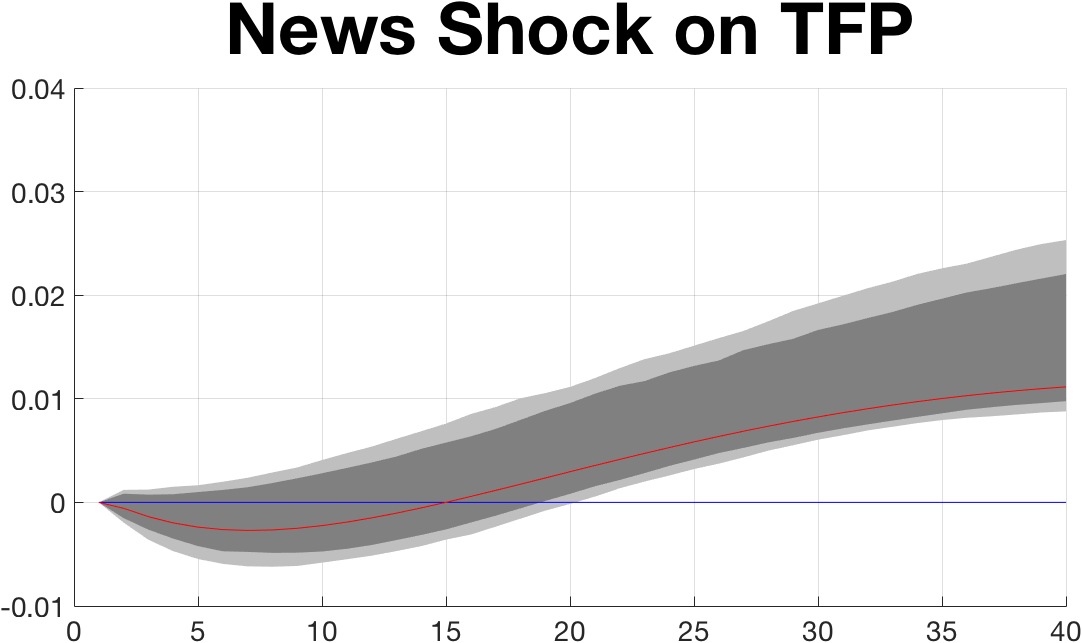
\includegraphics[scale=0.15]{\ourFigPath Figures/fig_News_Shock_on_TFP__} % REGENERATE TFP SHOCKS FIGURES WITH RIGHT SCALES!!
\end{figure}
\begin{figure}
	\centering
	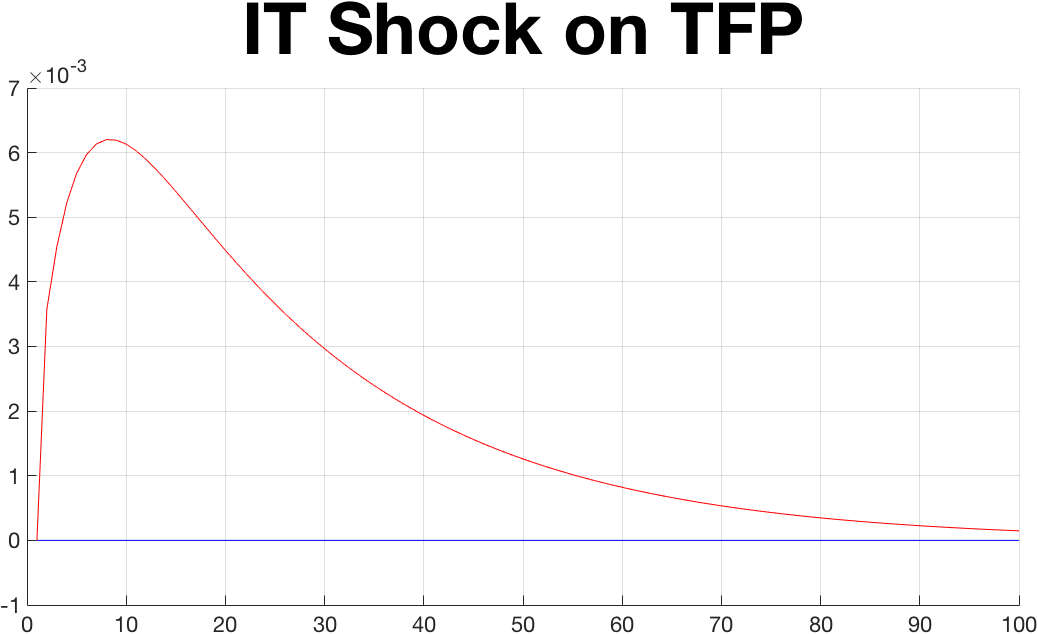
\includegraphics[scale=0.15]{\ourFigPath Figures/fig_IT_Shock_on_TFP__}
\end{figure}
\end{frame}
%%%%%%%%%%%%%%%%%%%%%%%%%%%%%

%%%%%%%%%%%%%%%%%%%%%%%%%
\begin{frame}
\frametitle{Real SP500 response to both shocks}
\begin{figure}
	\centering
	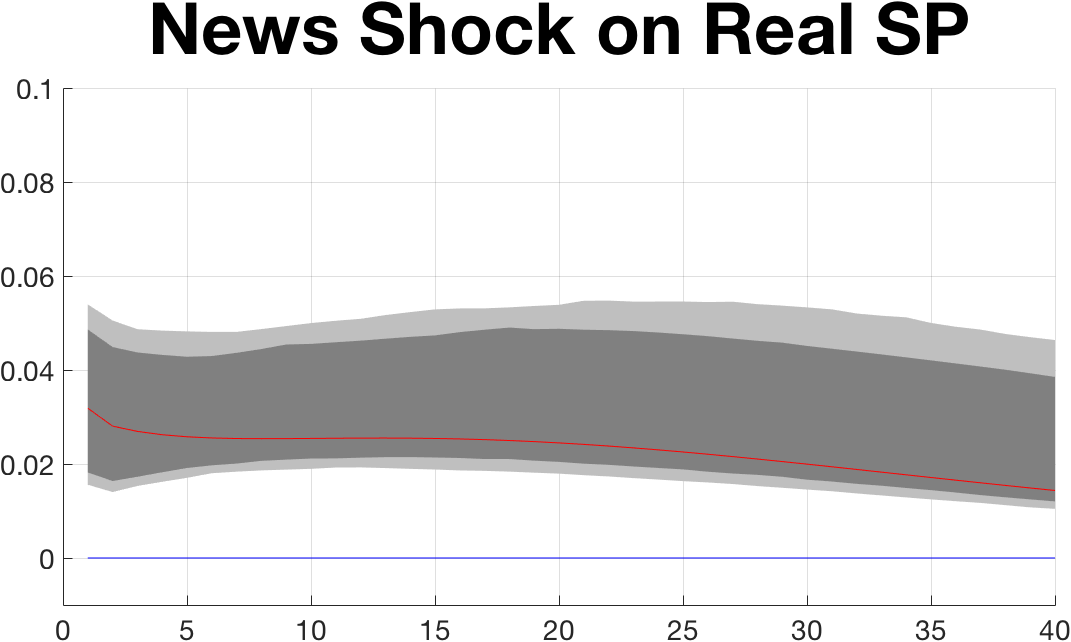
\includegraphics[scale=0.15]{\ourFigPath Figures/fig_News_Shock_on_Real_SP__}
\end{figure}
\begin{figure}
	\centering
	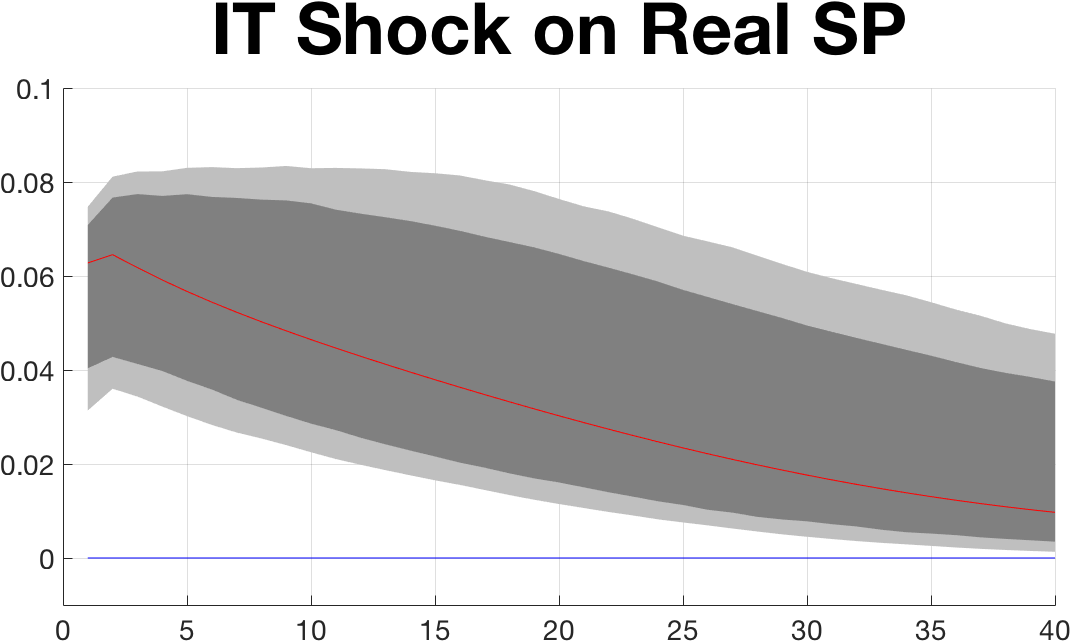
\includegraphics[scale=0.15]{\ourFigPath Figures/fig_IT_Shock_on_Real_SP__}
\end{figure}
\end{frame}
%%%%%%%%%%%%%%%%%%%%%%%%%%%%%

%%%%%%%%%%%%%%%%%%%%%%%%%
\begin{frame}
\frametitle{IT investment response to both shocks}
\begin{figure}
	\centering
	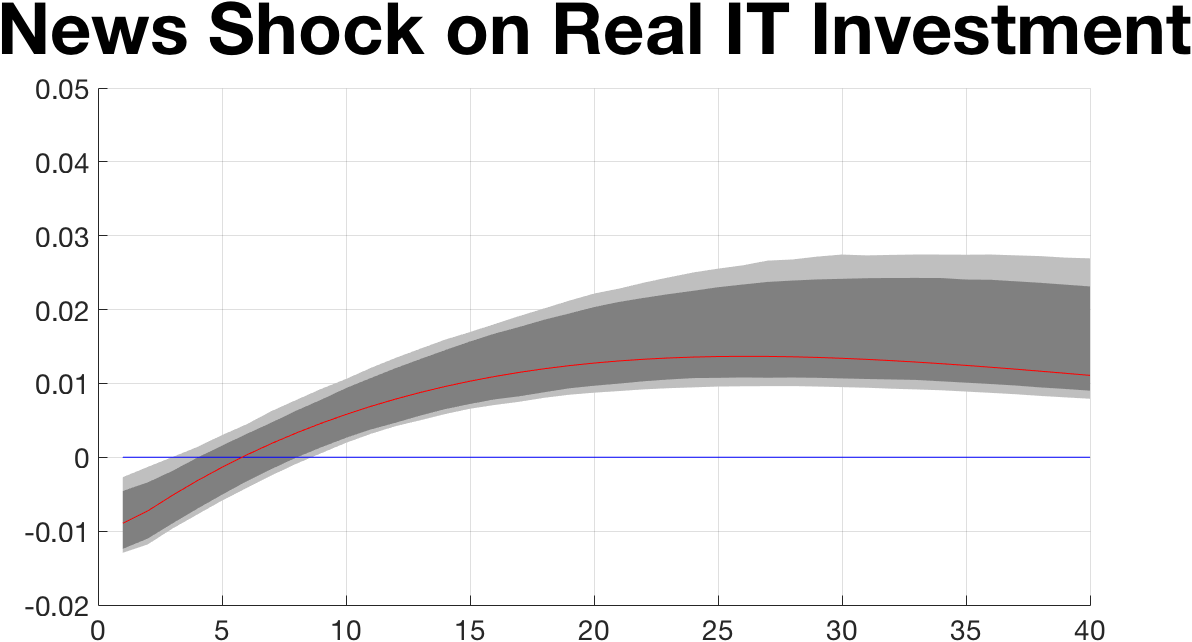
\includegraphics[scale=0.15]{\ourFigPath Figures/fig_News_Shock_on_Real_IT_Investment__}
\end{figure}
\begin{figure}
	\centering
	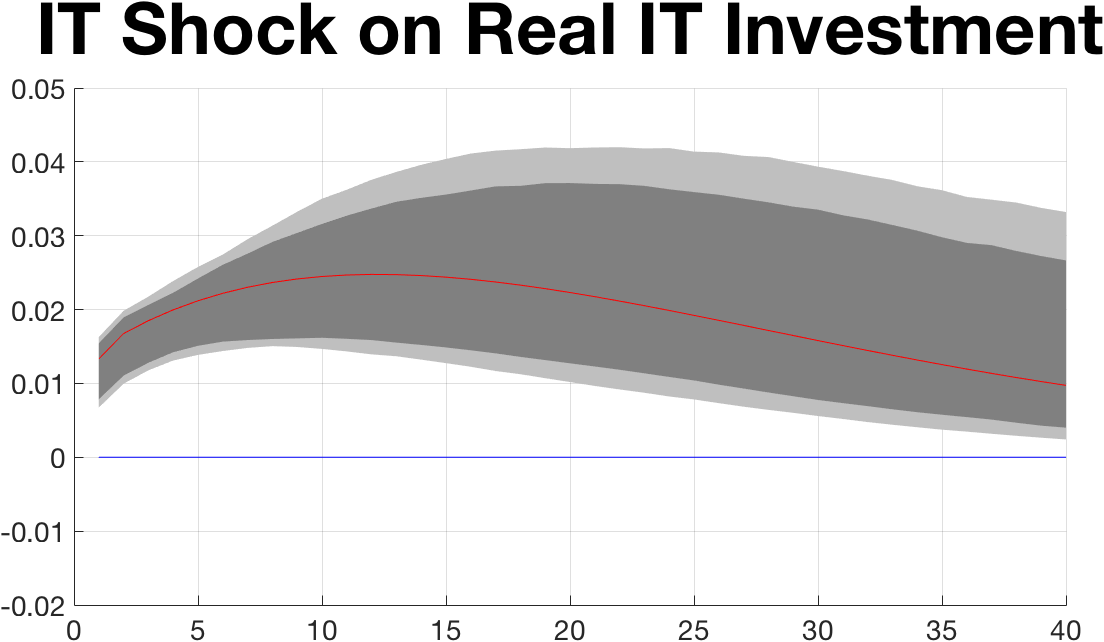
\includegraphics[scale=0.15]{\ourFigPath Figures/fig_IT_Shock_on_Real_IT_Investment__}
\end{figure}
\end{frame}
%%%%%%%%%%%%%%%%%%%%%%%%%%%%%


%%%%%%%%%%%%%%%%%%%%%%%%%
\begin{frame}
\frametitle{Other responses to both shocks}

\vspace{-0.2cm}
\begin{figure}
\begin{multicols}{2}
\centering 
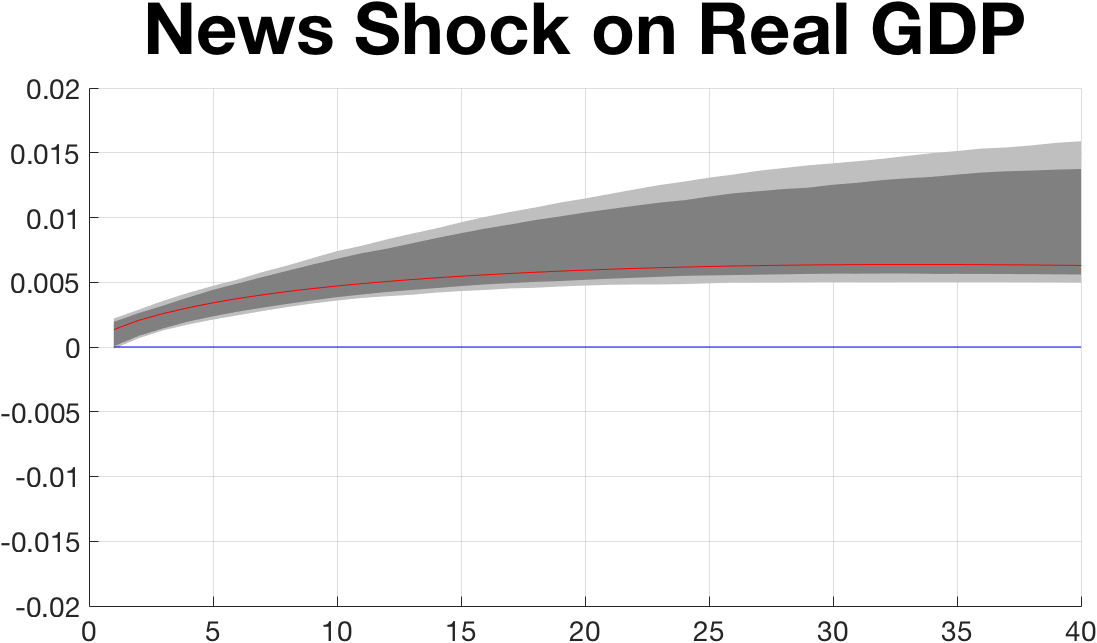
\includegraphics[scale = 0.1]{\ourFigPath Figures/fig_News_Shock_on_Real_GDP_Ryan_two_stepsID_10-Dec-2017_17_34_47}\\ 
\vspace{0.3cm}
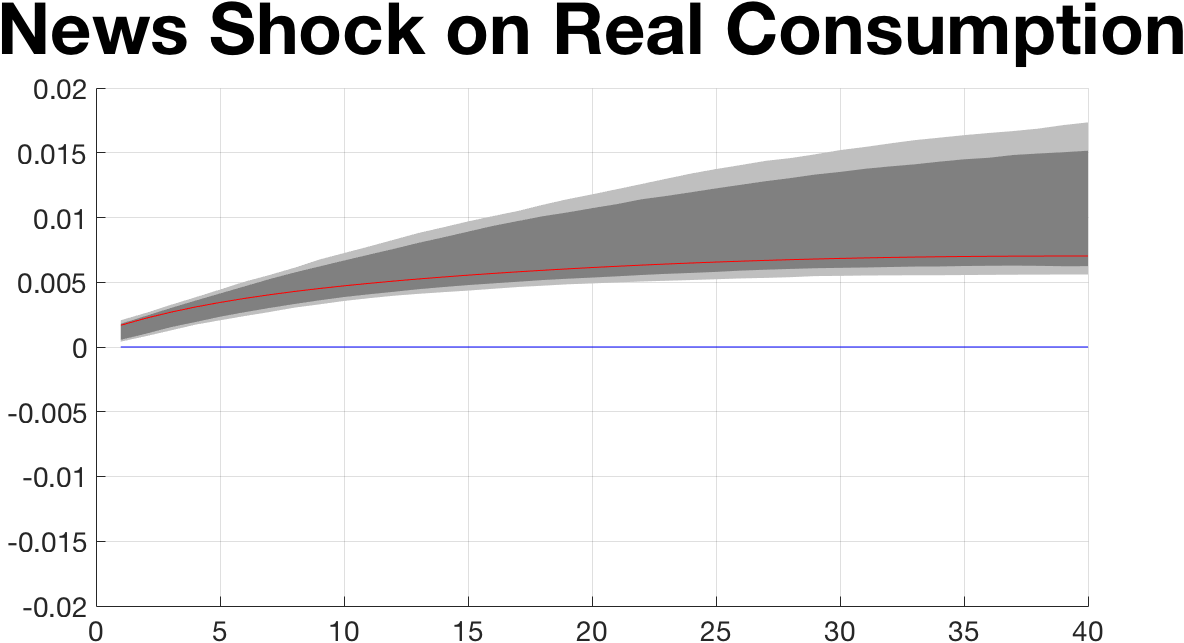
\includegraphics[scale = 0.1]{\ourFigPath Figures/fig_News_Shock_on_Real_Consumption_Ryan_two_stepsID_10-Dec-2017_17_34_50}\\ 
\vspace{0.3cm}
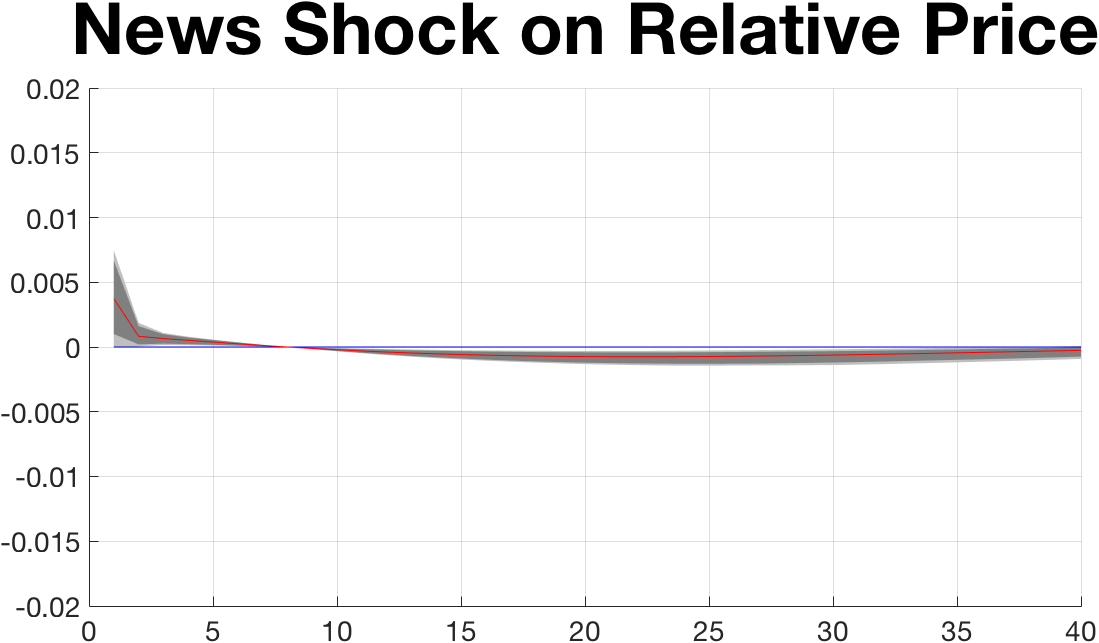
\includegraphics[scale = 0.1]{\ourFigPath Figures/fig_News_Shock_on_Relative_Price_Ryan_two_stepsID_10-Dec-2017_17_34_52}\\ 


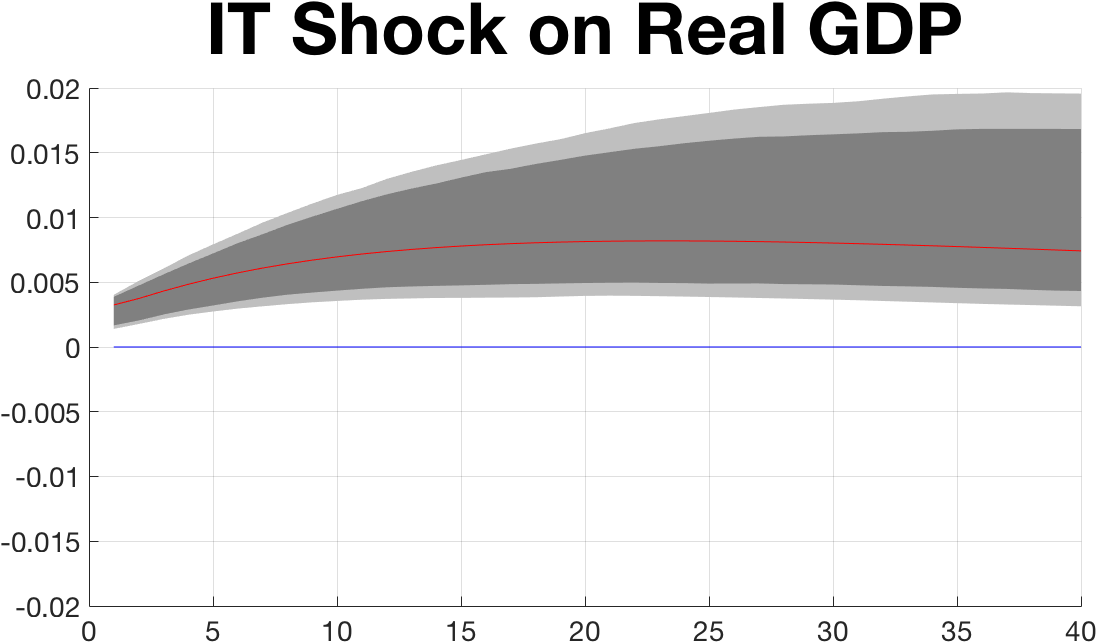
\includegraphics[scale = 0.1]{\ourFigPath Figures/fig_IT_Shock_on_Real_GDP_Ryan_two_stepsID_10-Dec-2017_17_35_00}\\
\vspace{0.3cm}
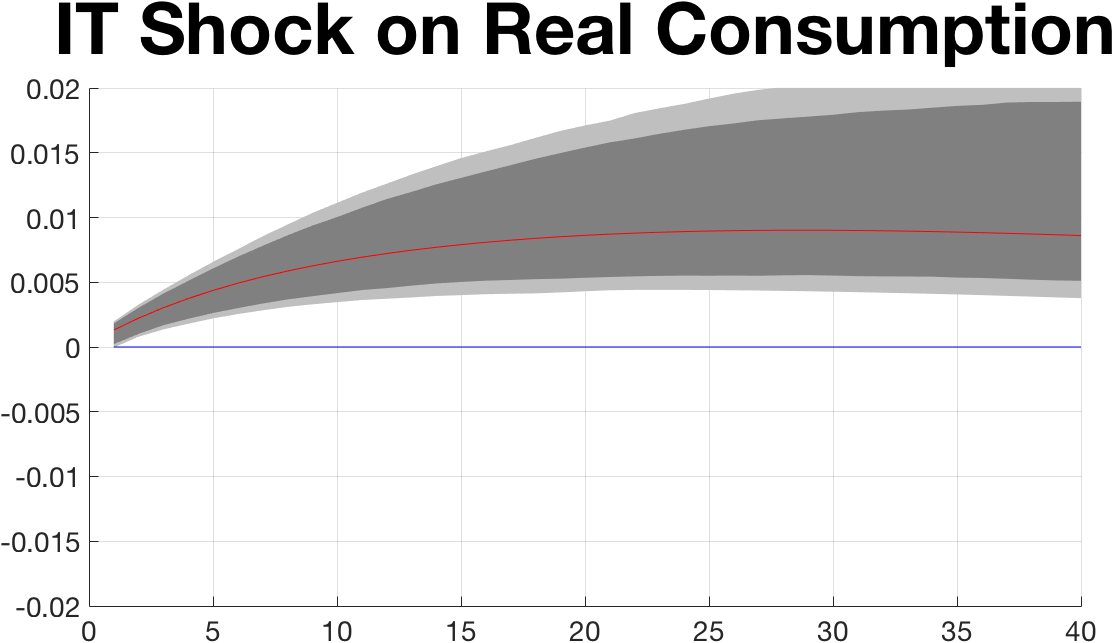
\includegraphics[scale = 0.1]{\ourFigPath Figures/fig_IT_Shock_on_Real_Consumption_Ryan_two_stepsID_10-Dec-2017_17_35_02}\\ 
\vspace{0.3cm}
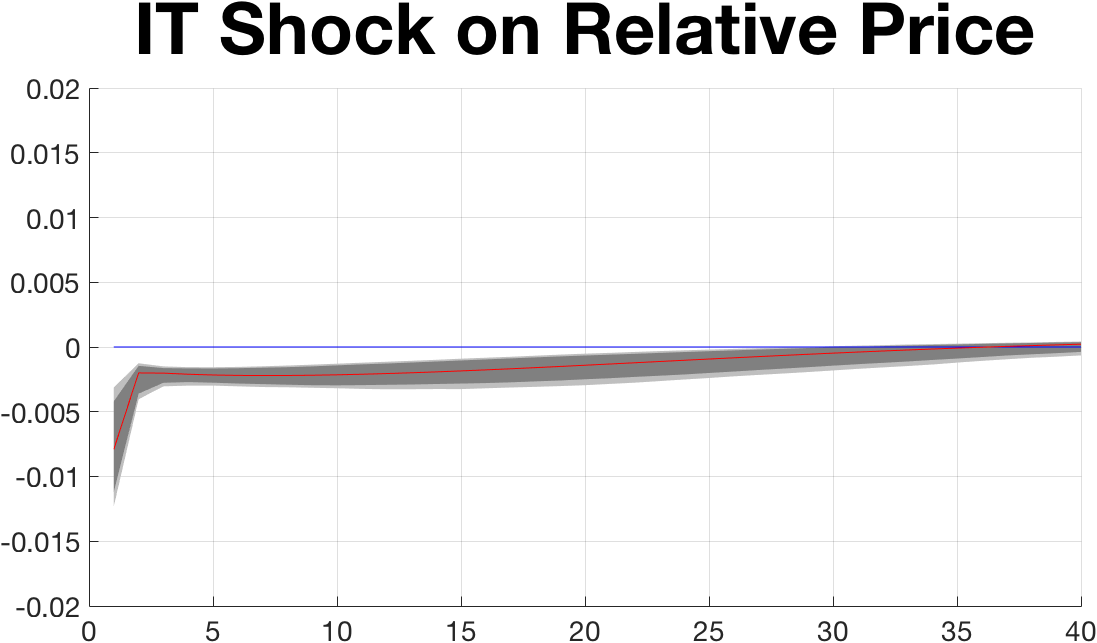
\includegraphics[scale = 0.1]{\ourFigPath Figures/fig_IT_Shock_on_Relative_Price_Ryan_two_stepsID_10-Dec-2017_17_35_04}\\ 

\end{multicols}
\end{figure}


\end{frame}
%%%%%%%%%%%%%%%%%%%%%%%%%%%%%


%%%%%%% Slide %%%%%%
\begin{frame}
	\frametitle{FEV explained by the two shocks at 60 periods}


    \hspace{2.25cm}
\begin{large}
	\begin{tabular}{lccc}
	\hline
		& News & IT & Total \\
		\hline
	TFP	           & 0.20384  & 0.52596 & 0.72981  \\
		\hline
	\end{tabular}
\end{large}

\vspace{2cm}

For BS, FEV of news was 45\%.
		 	
\end{frame}
%%%%%%%%%%%%%%%%%

%%%%%%% Slide %%%%%%
\begin{frame}
	\frametitle{Interpretation}

\begin{enumerate}
 \item Shape and timing of the responses reflect ...
 
 %\ 
 
	\begin{itemize}
	\item both the Barsky \& Sims result;
	
	\vspace{0.1cm}
	
	\item as well as the the conjecture that the IT shock looks similar to news along certain dimensions; 
	
	\vspace{0.1cm}
	
	\item but relative prices do indeed introduce a margin of difference between the two shocks.
	\end{itemize}

\

\item Shares of FEV of TFP explained ...
	\begin{itemize}
	\item are also in line with the Barsky \& Sims result;
	\item [] (for BS, news explains around 45\%, compared to 20\% here)
	
	\vspace{0.1cm}
	
	\item  yet suggest that the IT shock plays an important role as well (around 52\%).
	
	\vspace{0.1cm}
	
	\item And indeed the IT shock \emph{complements} the news shock, instead of substituting for it.
	\item [] For BS, the single identified shock explains around 45\%, while our two identified shocks explain around 73\%.
	\end{itemize}

\end{enumerate}
		 	
\end{frame}
%%%%%%%%%%%%%%%%%

%%%%%%% Slide %%%%%%
\begin{frame}
	\frametitle{Robustness checks}

\begin{itemize}
\item Different variables
	\begin{itemize}
	\item Add the Michigan index of consumer confidence (expected business conditions 5 years ahead)
	
	
	\
	
	\item Replace IT prices with capital prices (following Comin \& Gertler)
	\end{itemize}
	
	\
	
\item Different horizons at which we impose the restriction on relative prices for the news shock
\item[] $\rightarrow$ ran  6, 8, 10, 12 and 16 quarters.

\

\item Increase the number of lags (2)

\

\item Check whether VAR is information-sufficient to identify the news shock (Forni-Gambetti test) (p-val of 12\%)
\end{itemize}
   		 	
\end{frame}
%%%%%%%%%%%%%%%%%

%%%%%%% Slide %%%%%%
\begin{frame}
	\frametitle{A counterfactual} 

	\begin{figure}
		\centering
		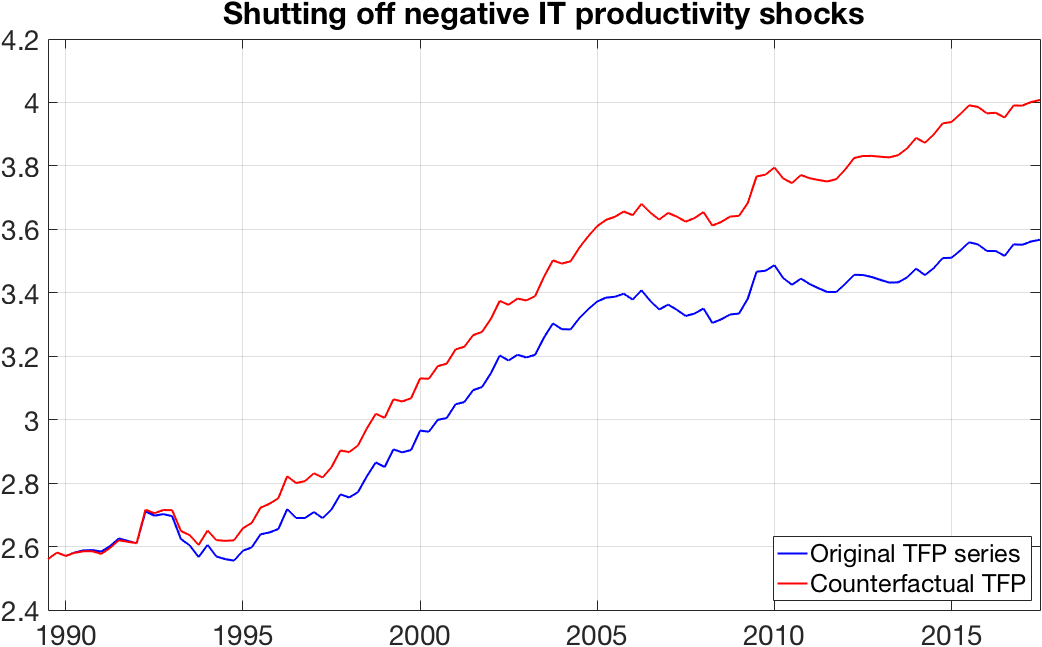
\includegraphics[scale=0.28]{\ourFigPath Figures/fig_counterfactual_}
	\end{figure}

	

   		 	
\end{frame}
%%%%%%%%%%%%%%%%%


%%%%%%% Slide %%%%%%
\begin{frame}
	\frametitle{Conclusion} 
	
\begin{itemize}
\item Provided a test for the role of IT as an example of GPTs in explaining fluctuations in long-run TFP, and in doing so, overcame an econometric challenge prevalent in the literature on long-run productivity.

\ 

\item The results show that by controlling for the presence of news shocks, IT productivity shocks are important drivers of TFP fluctuations at long horizons.

\

\item This result does not contrast however with the findings of the news shock literature since we still find that news also play a significant role in explaining TFP. 

\

\item Moreover, IT productivity shocks can be thought of as giving more microfoundations to what classical news shocks carry information on. 

\end{itemize}
   		 	
\end{frame}
%%%%%%%%%%%%%%%%%

%%%%%%% Slide %%%%%%
\begin{frame}
	\frametitle{Work ahead} 
	
\begin{itemize}

\item Show the identification assumption in the structural model. 

\

\item Technically, should do a VECM due to cointegration and wanting to have variables in the VAR as growth rates rather than levels...

\

\item Dig deeper: IT is just an example of GPTs for the last 30 years
\item[] $\hookrightarrow$ could redo analysis for different time periods with different GPTs (electricity in 1920s, airplane industry in 1960s ...)

\


\item Use a fully structural model to see if we can find interesting interactions between the two shocks?
\item [] $\hookrightarrow$ In particular, we're thinking of noise shocks on IT productivity

\	
	
\item But there are also other shocks that are similar to news shocks and yet not news shocks in the Barsky \& Sims sense: reallocative shocks, shocks to inventories, etc...  
\end{itemize}


   		 	
\end{frame}
%%%%%%%%%%%%%%%%%





%%%%%%%%%%%%%%%%%%%%%%%%%%%%%%%%%%%%%%%%%%%%%%%%%%%%%%%%%%%%%%%%%%%%%%
%%%%%%                     APPENDIX  
%%%%%%%%%%%%%%%%%%%%%%%%%%%%%%%%%%%%%%%%%%%%%%%%%%%%%%%%%%%%%%%%%%%%%%

%%%%%%% Slide %%%%%%
\begin{frame}
	\frametitle{The current TFP slowdown}
	
	
	\vspace{-1cm}
	\noindent
	\begin{figure}
		\centering
		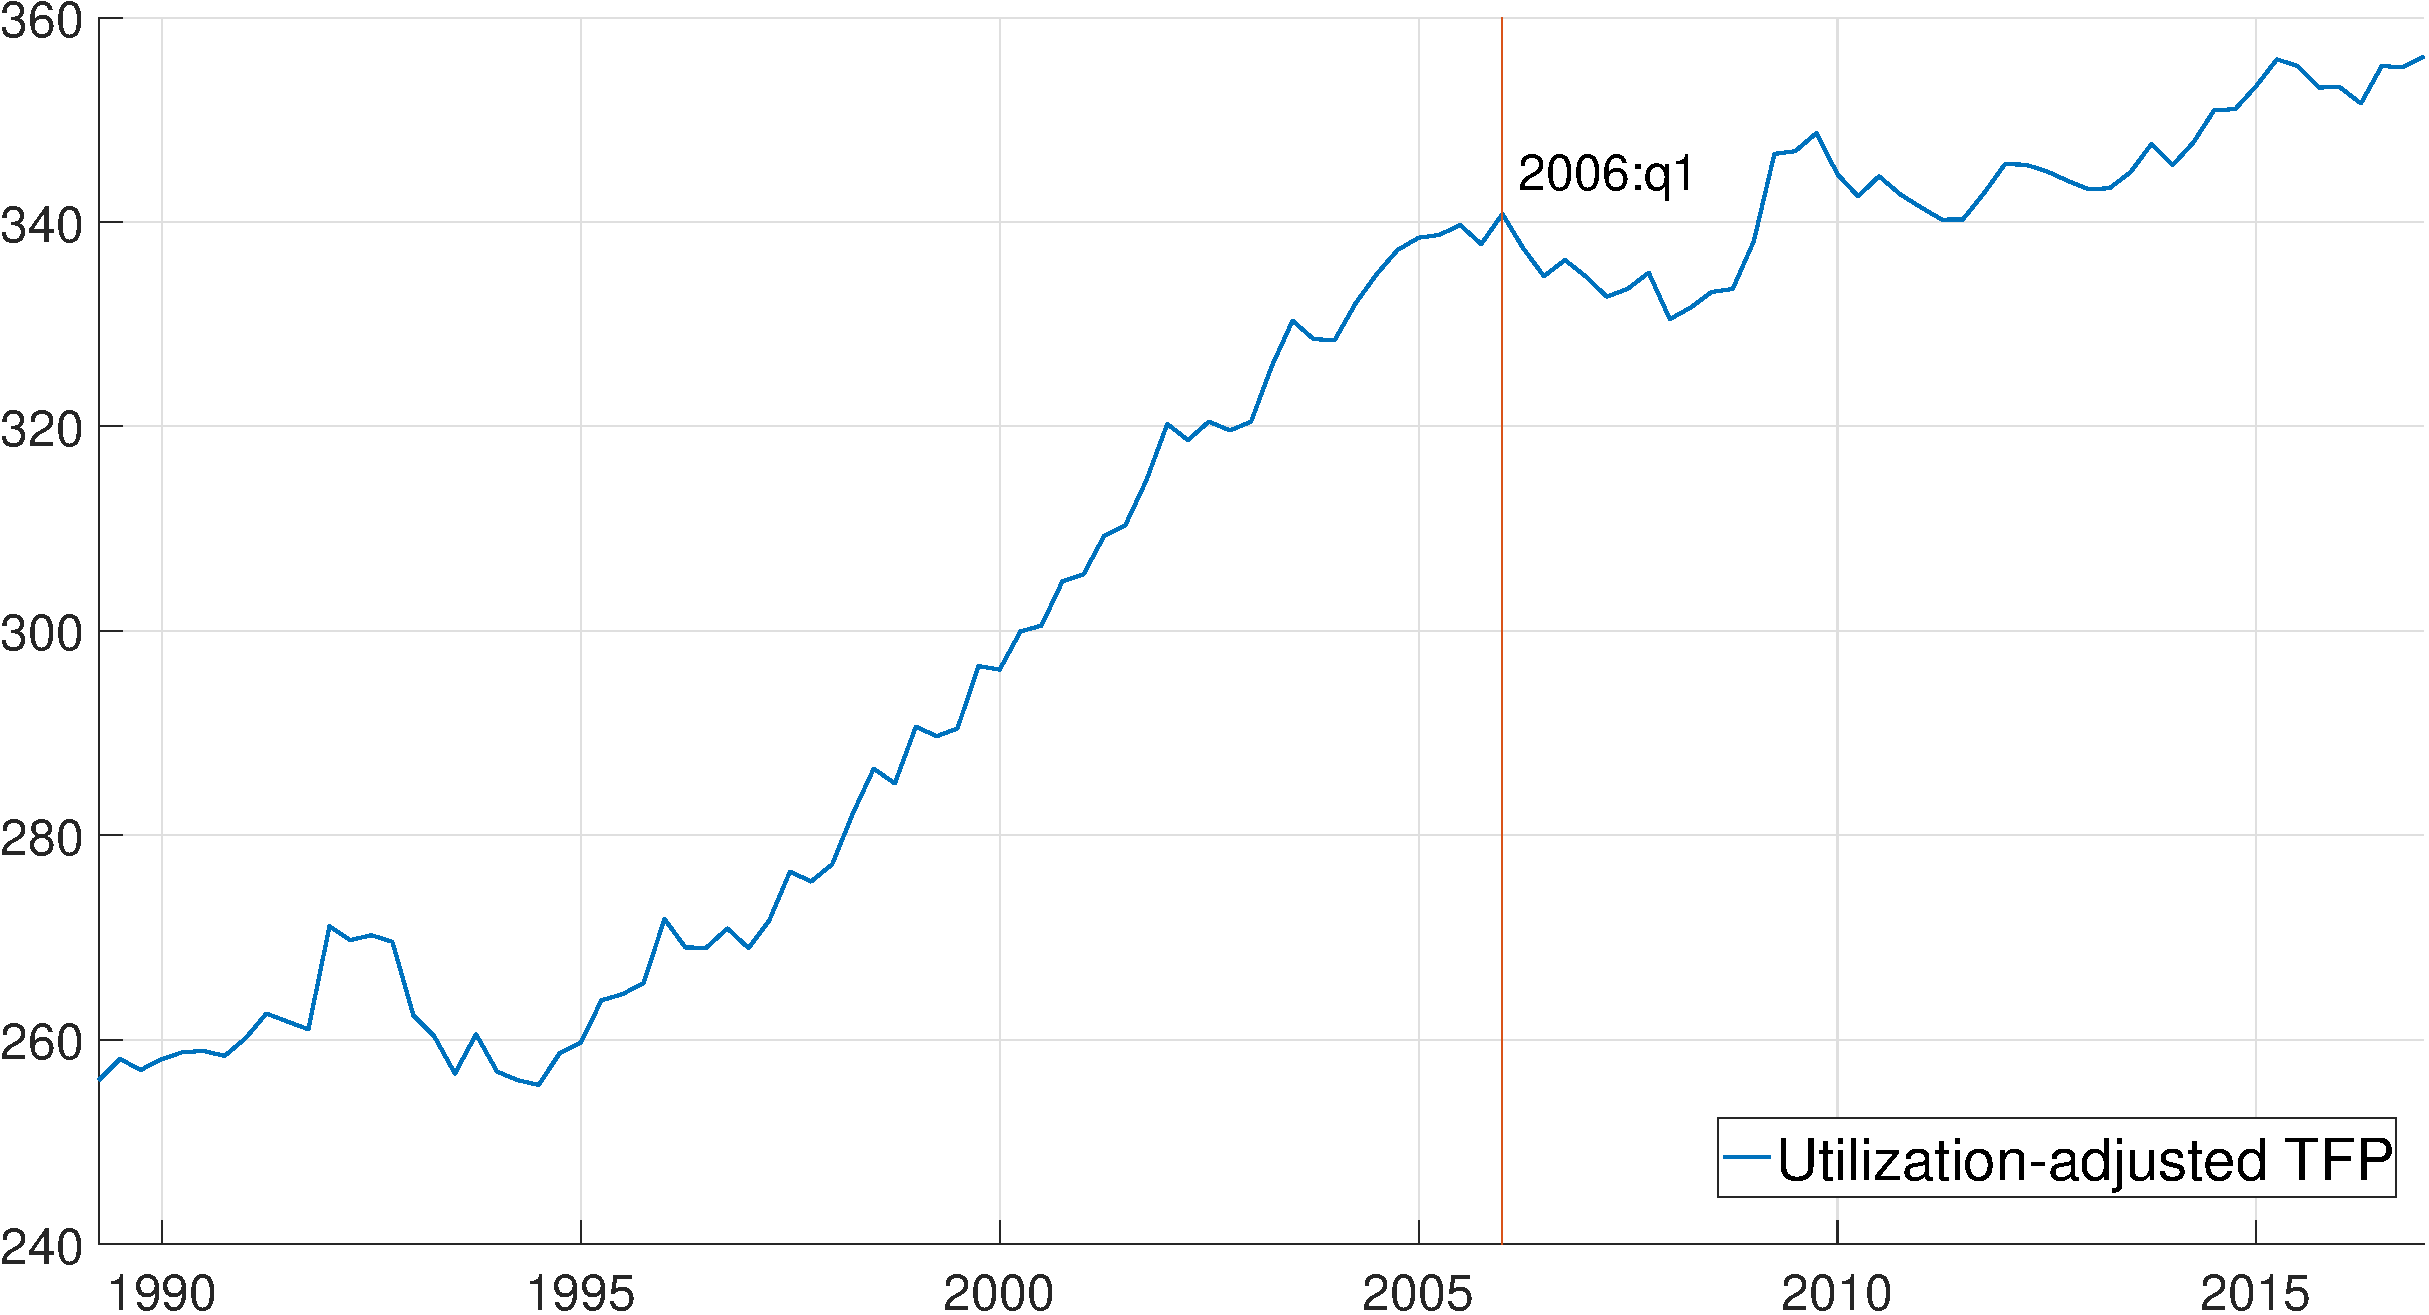
\includegraphics[scale=0.28]{\ourFigPath Figures/fig_TFP_macrolunch_29-Nov-2017_17_41_17}
	\end{figure}
	
	
\end{frame}
%%%%%%%%%%%%%%%%%


%%%%%%% Slide %%%%%%
\begin{frame}
	\frametitle{Barsky \& Sims FEV of TFP explained}
	\label{BS_FEV}
	

\vspace{-1cm}
\noindent
\begin{figure}
\centering
\includegraphics[scale=0.3]{\ourTablePath fig_BS_fevtable}
\end{figure}
	
\hyperlink{related_lit}{\beamerreturnbutton{Return}}	
\end{frame}
%%%%%%%%%%%%%%%%%

%%%%%%% Slide %%%%%%
\begin{frame}
	\frametitle{Production of IT goods}
	\label{it_sector}
	
Production function for IT goods:

\begin{equation}
V_{i,t} = \lambda_t \Psi_t f(S_{i,t}) 
\end{equation}
where $S_{i,t}$ is investment by producer $i$ in IT goods and $\lambda$ is the productivity of the IT sector. 

\

The IT producer's problem is to max discounted profits $J_{i,t+1}$

\begin{equation}
\max_{S_{i,t}} \; \mathbb{E}(\Lambda_{t,t+1},J_{i,t+1})\lambda_t \Psi_t f(S_{i,t}) - P^{IT}_t S_{i,t}
\end{equation}

\
FOC: 

\begin{equation}
P^{IT}_t = \mathbb{E}(\Lambda_{t,t+1},J_{i,t+1})\lambda \Psi_t f_1
\end{equation}
	
\hyperlink{expanding_variety}{\beamerreturnbutton{Return}}	
\end{frame}
%%%%%%%%%%%%%%%%%


%%%%%%% Slide %%%%%%
\begin{frame}
	\frametitle{Timing: RD drop vs TFP drop}
	\label{timing}
	
	\vspace{-1cm}
	\noindent
	\begin{figure}
		\centering
		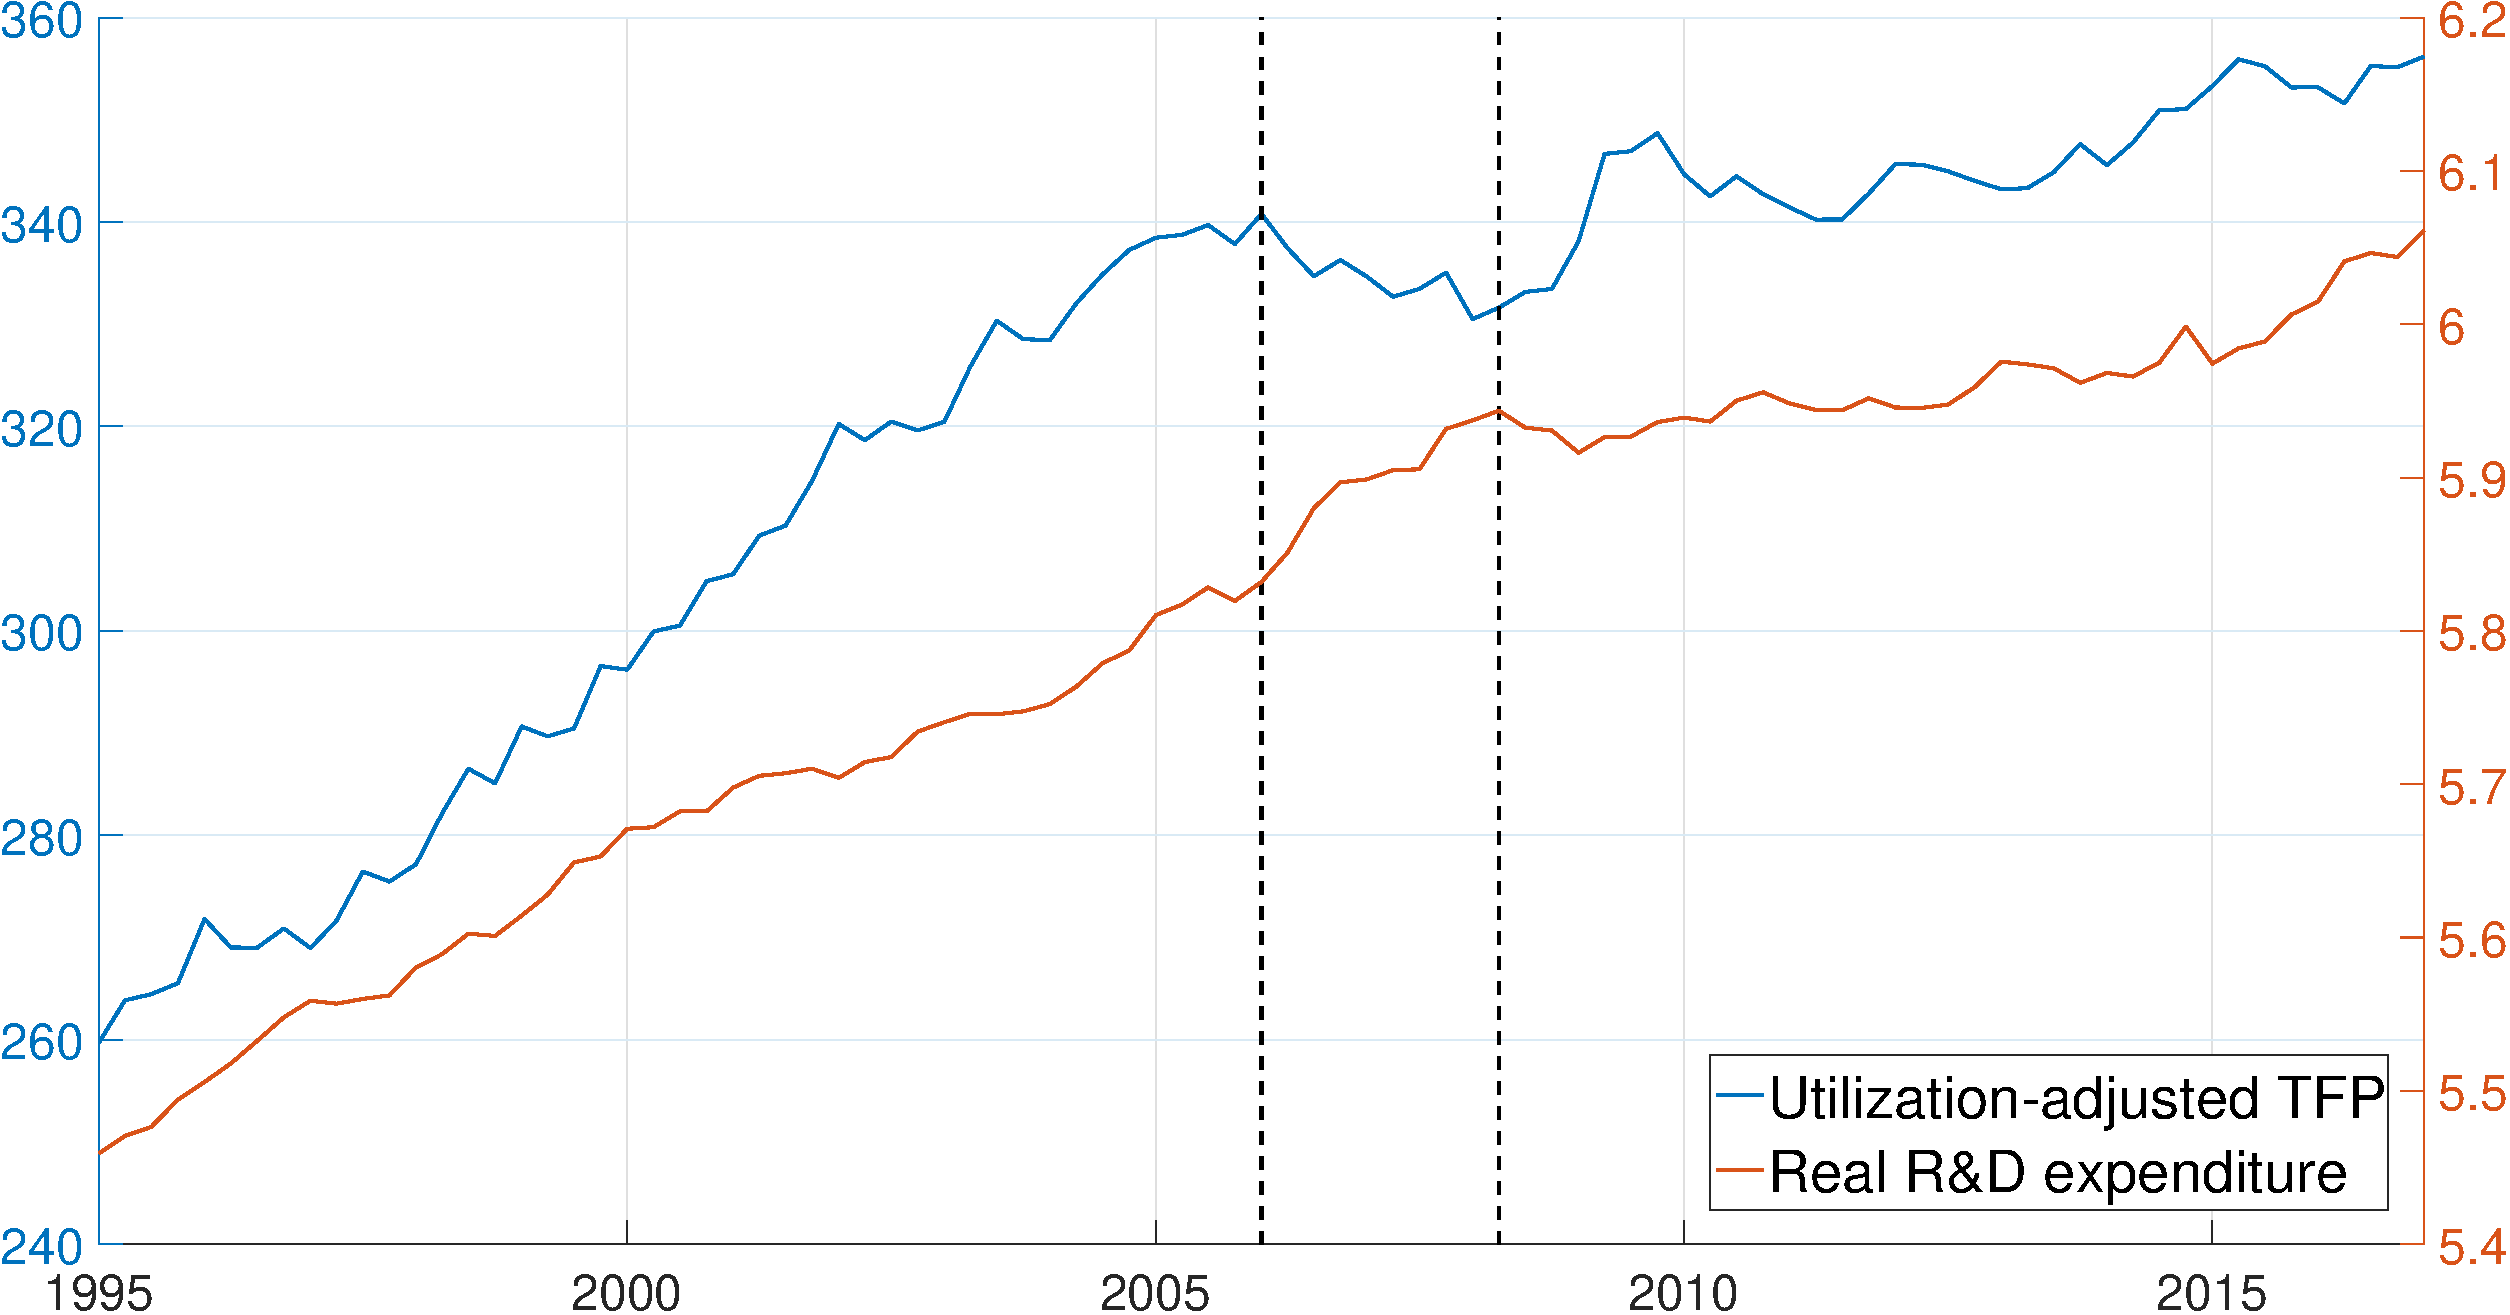
\includegraphics[scale=0.28]{\ourFigPath Figures/fig_RD_level_macrolunch_30-Nov-2017_11_31_04}
	\end{figure}

	
\hyperlink{convincing}{\beamerreturnbutton{Return}}	
\end{frame}
%%%%%%%%%%%%%%%%%

%%%%%%% Slide %%%%%%
\begin{frame}
	\frametitle{IT investment: a drop at the right time}
	\label{it_investment}
	
%	\vspace{-1cm}
	\noindent
	\begin{figure}
		\centering
		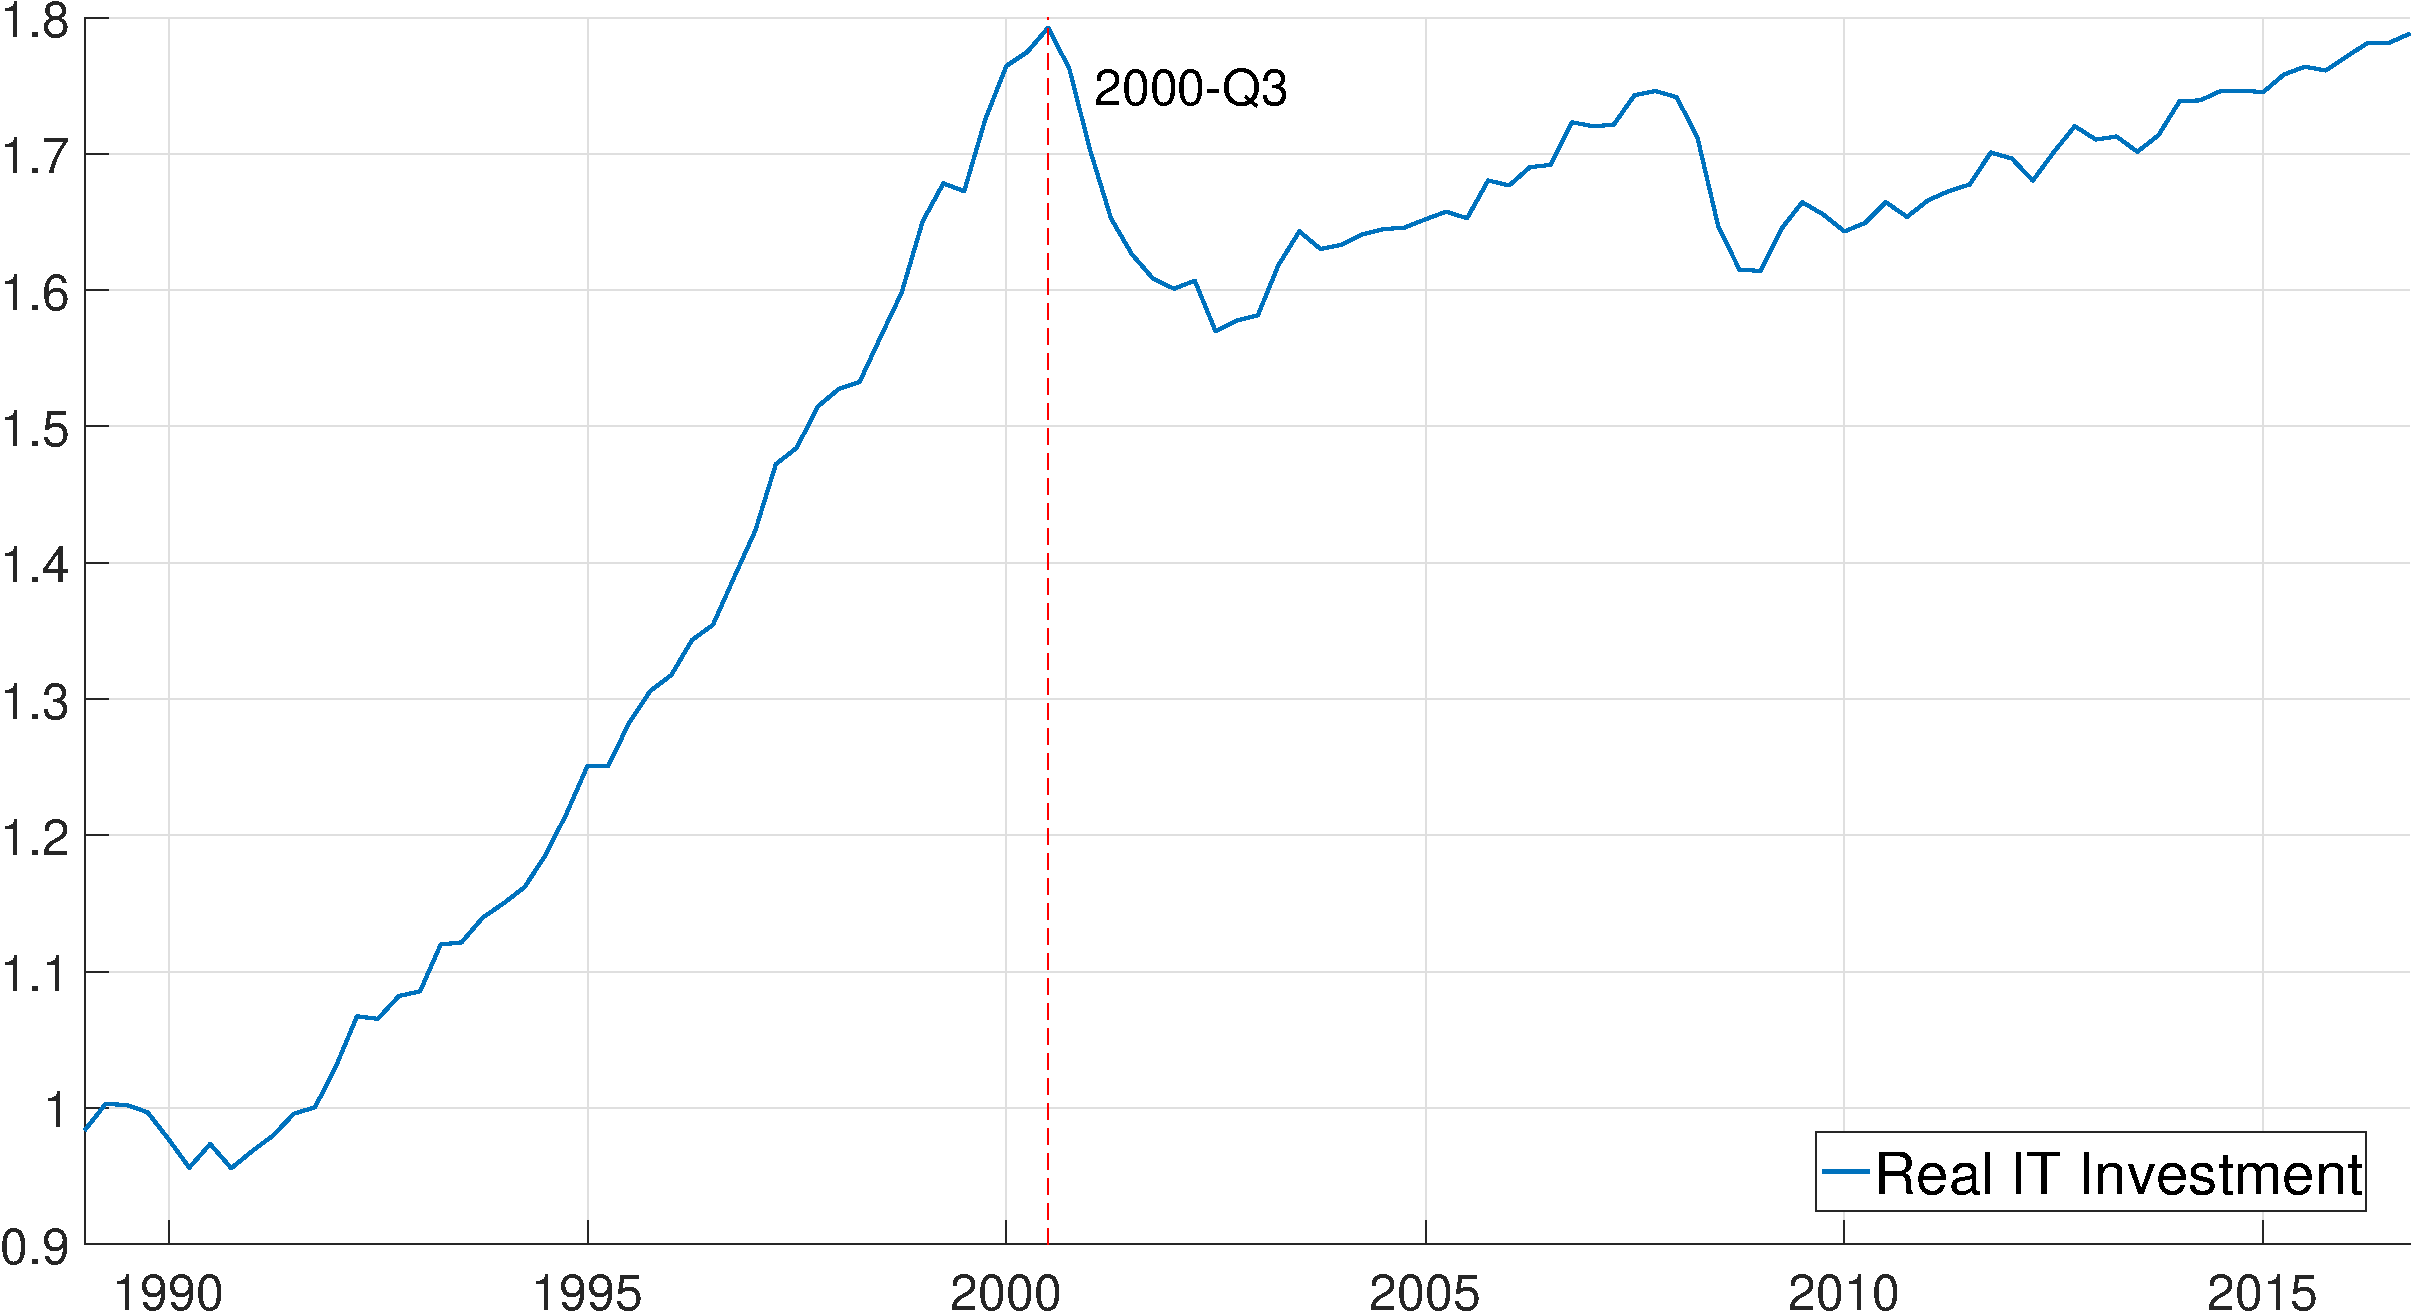
\includegraphics[scale=0.29]{\ourFigPath Figures/fig_IT_level_macrolunch_30-Nov-2017_11_37_26}
	\end{figure}

	
\hyperlink{convincing}{\beamerreturnbutton{Return}}	
\end{frame}
%%%%%%%%%%%%%%%%%

%%%%%%% Slide %%%%%%
\begin{frame}
\frametitle{Identification Strategy}
\label{Technicalities}

\begin{equation}
D = \begin{bmatrix}
d_{11} & \gamma_{12} & \gamma_{13} & d_{14} & \cdots \\
d_{21} & \gamma_{22} & \gamma_{23} & d_{24} & \cdots \\
\vdots & \vdots & \vdots & \ddots & \vdots 
\end{bmatrix}
\end{equation}

\begin{itemize}
	\item Indifferent over $d_{ij}$ as long as $D$ is orthogonal
	\item $A \gamma_{2}$ is the impact response to a news shock
	\item $A \gamma_{3}$ is the impact response to a IT productivity shock
	\item First element of both $A \gamma_{2}$ and $A \gamma_{3}$ is zero due to the no-contemporaneous effect of both shocks on TFP
	\item $A \gamma_2$ is such that the FEV of TFP is maximized subject to zero long-run effect on $RP$
	\item $A \gamma_3$ is maximizing the remaining FEV of TFP 
\end{itemize} 


\hyperlink{identification}{\beamerreturnbutton{Return}}	
\end{frame}
%%%%%%%%%%%%%%%%%
	
	





















\end{document}
